\chapter{Teoretická část} % Je to vhodný název kapitoly?

\section{Testování}

Testování je podstatnou součástí vývoje softwaru. Cílem testování není pouze odhalení chyb v softwaru, ale také verifikace a validace softwaru \cite{singh2012software}. Při testování se snažíme vytvářet situace, ve kterých můžeme ověřit, že se software chová dle zadané specifikace.

Testování softwaru je zároveň dovednost \cite{fewster1999software}. Při testování musí tester vybrat z nekonečného množství možných testů nějaký konečný počet, který nejlépe reprezentuje danou problematiku a pokrývá co největší možnou množinu všech možných případů. Zároveň musí vzít v potaz náročnost na vytvoření testu a na rigidnost vytvořeného testu proti změnám v softwaru. Tyto faktory poté ovlivňují i náklady na testování. 

Od testování softwaru se také odvodit kvalita softwaru. Kvalitu softwaru se dá určit tím, jak moc vytvořený software odpovídá zadaným specifikacím \cite{software_quality}. Tyto informace jsou poté velmi důležité pro managment. Díky nim může vyhodnocovat současný stav vývoje a upravovat plán na vývoj. 

Testování zároveň zvyšuje důvěru ve vyvíjený softwaru. Každý dobře navržený test snižuje šanci, že v softwaru existuje nepodchycená chyba. S každým rozsáhlým testováním se tato důvěra zvyšuje \cite{fewster1999software}.



\subsection{Rozdělní testů}

I když cíl testování je jednotný, přístupů k testování je několik. Vhodnost jednotlivých přístupů se mění na základě testované komponenty. Tyto přístupy se dají rozdělit do několika kategorií \cite{luo2001software}.

\subsubsection{Podle znalosti komponenty}

Testování se dá rozdělit podle přístupu k informacím, které o komponentách softwaru/systému víme. Tyto typy jsou:

\begin{description}
    \item[Black box testování] Nazýváno taktéž funkční testování. Na software se pohlíží jako na tzv. černou skříňku. O komponentě nebo celku nic nevíme a testujeme na základě funkcionálních požadavků a návrhu. 
    \item[White box testování] Se znalostí implementace testované části se snažíme vytvořit takové testy, které způsobí spouštění určitých částí testované komponenty. Cílem je co největší pokrytí testování dané komponenty.
    \item[Grey box testování] Kombinace Black box a White box testování. Při testování máme nějakou znalost implementace komponenty, ale je nižší, než při White box testování \cite{khan2010different}.
\end{description}

\subsubsection{Podle částí vývoje}

Testování podle částí vývoje se přibližuje vývojovému cyklu. Tyto kategorie jsou:  

\begin{description}
    \item[Testování částí] V angličtině nazýváno známým pojmem \uv{Unit testing}. Je to nejnižší úroveň testování. Testuje jednotlivé komponenty systému samostatně.
    \item[Integrační testování] Testování dvou a více komponent, které spolu vytváří nějaký větší celek softwaru. Často také využíván při testování částí, které nelze samostatně testovat.
    \item[Systémové testování] Testování softwaru jako celku. Testování se směřuje na testování funkčních požadavků. Zároveň je možno vyhodnocovat další požadavky na systém, jako spolehlivost, bezpečnost, atd.
    \item[Akceptační testování] U toho testování se systém dostane do rukou zákazníkovi/uživatelům. Cílem je otestování produktu u potencionálních uživatelů softwaru a získání jejich zpětné vazby. 
\end{description}

Propojení testů a vývojového cyklu je dobře znázorněno na tzv. V-modelu, který můžeme vidět na obrázku \ref{fig:vmodel}. Na tomto modelu, nazývaném podle svého tvaru, můžeme vidět jednotlivé typy stádia vývoje a korespondující jejich ověřování v závislosti na čase.

\begin{figure}[htbp]
    \centering 
    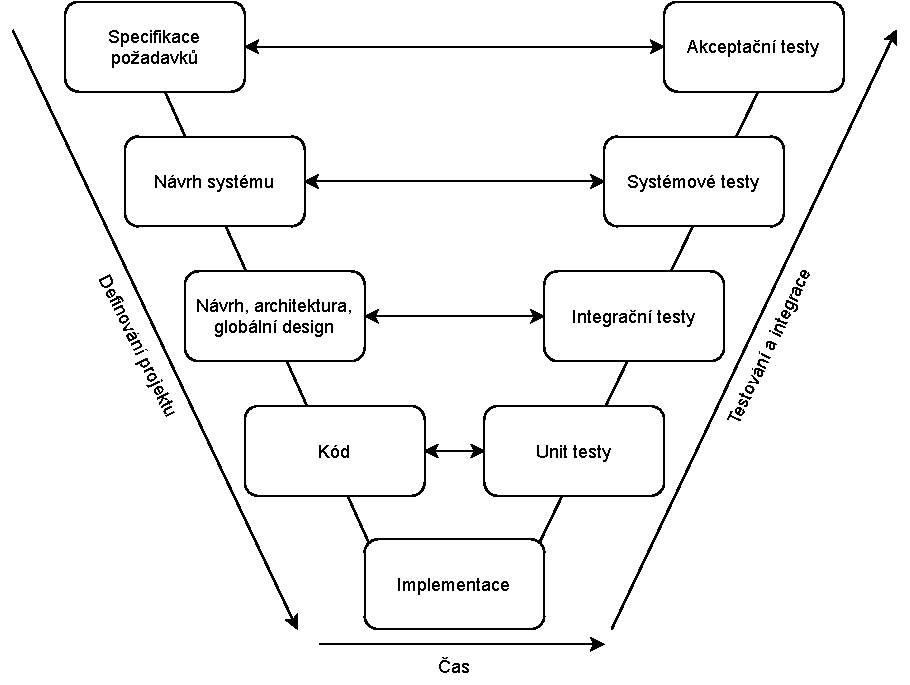
\includegraphics[width=0.9\textwidth]{assets/img/vmodel.pdf}
    \caption{V-model \question{Je potřeba citovat}}
    \label{fig:vmodel}
\end{figure}



\subsubsection{Analýza softwaru}
Součástí testování je i analýza softwaru. Tato analýza se dá rozdělit podle toho, zda je potřeba daný vyvíjený software vůbec spouštět. Tyto kategorie jsou:

\begin{description}
    \item[Statická analýza] Tato analýza je prováděno bez spuštění softwaru. Analýza je prováděna na napsaný kód. Vyhodnocovány jsou obecné vlastnosti napsaného kódu bez znalosti kontextu použití.
    \item[Dynamická analýza] Testování je provedeno spuštěním softwaru a použitím reálných metod systému s reálnými daty v simulovaných situacích. 
\end{description}

\section{Automatizace testování}

Automatizace testování je odlišná od samotného testování. Automatizace testu neurčuje samotnou kvalitu testu. Pokud automatizujeme test, který nic nového nepřinese, dostaneme toto nic pouze rychleji \cite{fewster1999software}. Automatizování je ale přesto v mnoha ohledech v dnešní době standardem při testování, a to především díky jeho výhodám. Mezi tyto výhody podle \cite{fewster1999software} patří:

\begin{description}
    \item[Častější testování] S automatizací jsme schopni testovat software mnohem častěji, než při manuálním testování. Software může být testován například při každé jeho změně. Toto manuálně je velmi náročné, už jenom kvůli vysokému požadavku na lidské zdroje.  
    \item[Možnost testovat nové věci] Automatizace umožňuje testovat takové aspekty, které se nedají manuálně testovat, nebo jejich manuální testování je velice náročné. Tím se zvyšuje pokrytí testování.
    \item[Lepší využití zdrojů] Tester je vysoce kvalifikovaný člověk a jeho využití na opakované vkládání vstupů a ověřování výstupů je v některých případech plýtvání jeho drahocenným časem. Díky automatizaci se tester může zaměřit na jiné přínosnější činnosti, jako například vytváření nových testů, kterými pokryje nové případy.
    \item[Konzistence] Při automatizaci testování každý běh testu proběhne naprosto identicky. Stejně jako ve vývoji, i v testování může dojít k lidské chybě. Díky automatizaci se šance lidské chyby snižuje. Toto zvyšuje konzistenci testování, než když se testy provádějí manuálně.
    \item[Snížení doby testování] Jednou automatizované testy můžou být provedeny mnohem rychleji a efektivněji, než při jejich manuálním spuštění. Toto způsobuje snížení potřebné doby na testování.
\end{description}



% Díky automatizaci jsme při vývoji schopni provádět opakované testy za frakci ceny, než kdyby byli prováděny manuálně. Toto zároveň uvolňuje testery ke směřování své snahy k rozšiřování množiny testů a tím pokrytí co nejvíce případů. 

\todo{Rozšíření textu o automatizaci}


\section{Průmyslová komunikace}

Při řešení průmyslové komunikace se často objevuje slovo \textit{fieldbus}. Běžný význam tohoto slova je \uv{Síť, která propojuje průmyslová zařízení jako kontrolery, PLC, regulátory atd.} \cite{fieldbus_thomesse}. Vznik těchto sítí je úzce spojený s historií vývoje informačních technologií. V době, kdy začali tyto sítě vznikat, nebyli dostupné komunikační technologie, jako dnes. Dostupné informační a telekomunikační sítě té doby nemohli uspokojit potřeby průmyslových sítí na deterministickou, spolehlivou a efektivní komunikaci \cite{future_of_ind_com}. 

V dnešní době jsou tyto průmyslové sítě mezinárodně standardizovaný. Jako příklad protokolů můžeme uvést ModbusTCP, nebo Ethernet/IP, které už využívají výhod Ethernet připojení a zároveň satisfakují průmyslové potřeby. 
